\documentclass[12pt,a4paper]{article}
\usepackage[utf8]{inputenc}
\usepackage{geometry}
\geometry{margin=1in}
\usepackage{enumitem}
\usepackage{hyperref}
\usepackage{graphicx}
\usepackage{float}
\usepackage{pdfpages}
\usepackage{titlesec}
\usepackage{tabularx}
\usepackage{booktabs}
\usepackage{array}
\usepackage{float}


\titleformat{\section}{\large\bfseries}{\thesection.}{0.5em}{}

\begin{document}

% ============================================================
% TITLE PAGE
% ============================================================
\begin{center}
    {\Huge \textbf{Kalamna - AI Customer Support Egyptian Service}}\\[0.8cm]

    {\large \textbf{Supervisors:} Dr. Ahmed Yousry \& Eng. Mahmoud Sobhy}\\[0.3cm]

    {\large Faculty of Computer Science, Benha National University}\\[0.3cm]
    {\large Academic Year: 2025–2026}\\[0.3cm]

    {\small \textbf{Team Members:} Bassant Hossam, Ahmed Ehab Elattar, Eyad Hesham,\\ 
    Zeyad Wael, Shahda Mohamed, Toni Ehab}\\[0.8cm]
\end{center}

% ============================================================
% 1. IDEA DESCRIPTION
% ============================================================
\section{Idea Description}
Our project is an AI-powered, customizable Arabic “Egyptian” customer support platform designed to help SMEs automate their customer service across channels like WhatsApp, Messenger, and web platforms by integrating our service.

\textbf{Main Features:}
\begin{itemize}[noitemsep]
    \item Understanding of the Arabic dialect of Egypt.
    \item Customization \& rule for answers.
    \item Text support.
    \item Voice support (speech-to-text \& text-to-speech).
    \item Real-time emotion detection.
    \item Multi-intent handling.
    \item Integrations: WhatsApp, Messenger, Websites, Apps.
\end{itemize}

% ============================================================
% 2. PROBLEM STATEMENT
% ============================================================
\section{Problem Statement}
\textbf{Local businesses struggle with:}
\begin{itemize}[noitemsep]
    \item Providing consistent, 24/7 customer support.
    \item Repetitive questions.
    \item Missed messages.
    \item Slow response times.
\end{itemize}

All this leads to poor customer satisfaction. Existing solutions are often expensive, rigid, or lack authentic local language and dialect support.

% ============================================================
% 3. PROPOSED SOLUTION
% ============================================================
\section{Proposed Solution}
\textbf{We aim to build a flexible, API-powered Agent/Services system that:}
\begin{itemize}[noitemsep]
    \item Uses advanced AI Models \& APIs (Gemini, GPT, Whisper) for text, voice, and emotion-aware replies.
    \item Supports the Egyptian dialect as a primary focus.
    \item Detects user emotions and adapts responses accordingly.
    \item Allows businesses to fully customize the bot’s tone, responses, and operating hours.
\end{itemize}
\section{Prototype \& Identity}
We are currently developing the prototype. The chatbot will be named \textbf{Cleo} (short for \textit{Cleopatra}), and the overall service will be called \textbf{Kalamna}.  
Our chosen theme blends \textbf{Ancient Egyptian aesthetics} with an \textbf{Arabic-focused} design direction.  
We are now working on a sample prototype that will later be updated to fully reflect our visual identity.

\textbf{Figma Link:} \textit{(Pending link)}

% ============================================================
% 4. SYSTEM ANALYSIS
% ============================================================
\section{System Analysis Diagrams}
We are currently in the system analysis phase.  
The following diagrams represent our vision and planned design.
\begin{itemize}
    \item Flowcharts for user and business Flow
    \item ERD 
    \item sequence User diagram 
    \item sequence Business diagram
    \item DFD Level 0 "Context" 
    \item DFD Level 1 "User Flow" 
    \item DFD Level 2 "User Flow" 
    \item DFD Level 1 "Business Flow"
    \item High level system design \& Arch Diagram >> PNG Version not here
    \item UseCase User and Business Diagram
\end{itemize}

with that we also working on prototype for widget and dashboard

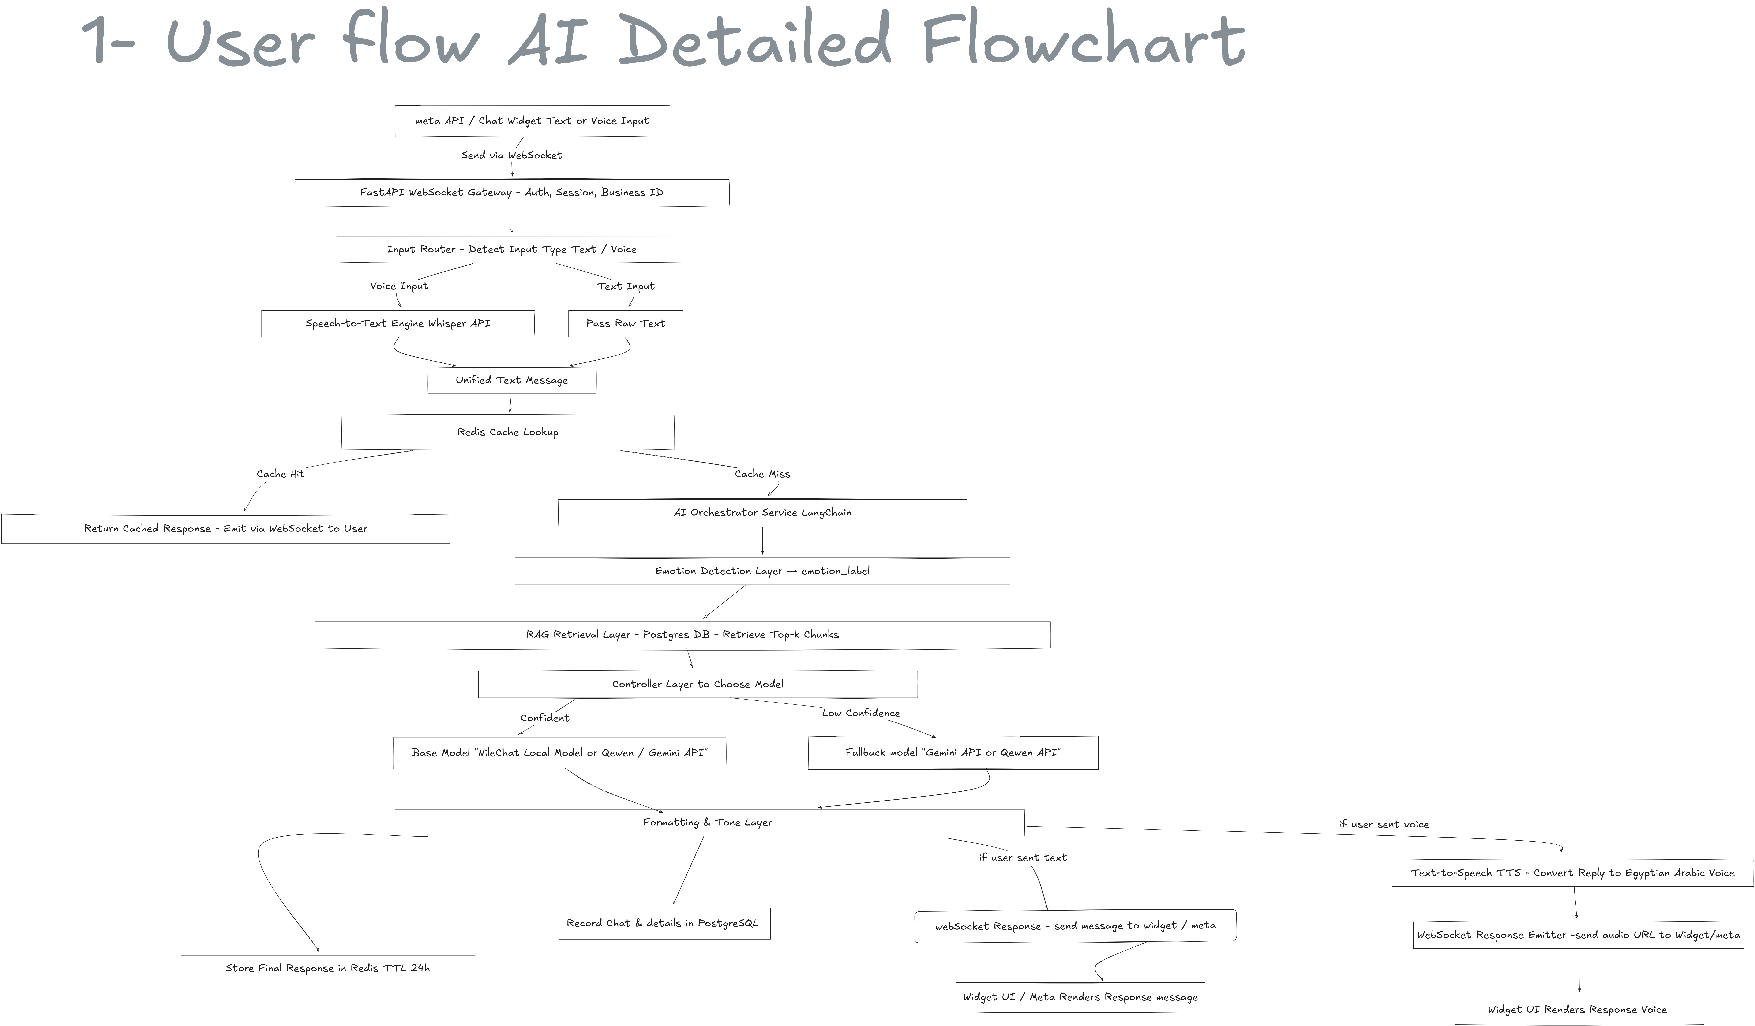
\includepdf[pages=-, fitpaper=true]{User Flow AI layer.pdf}
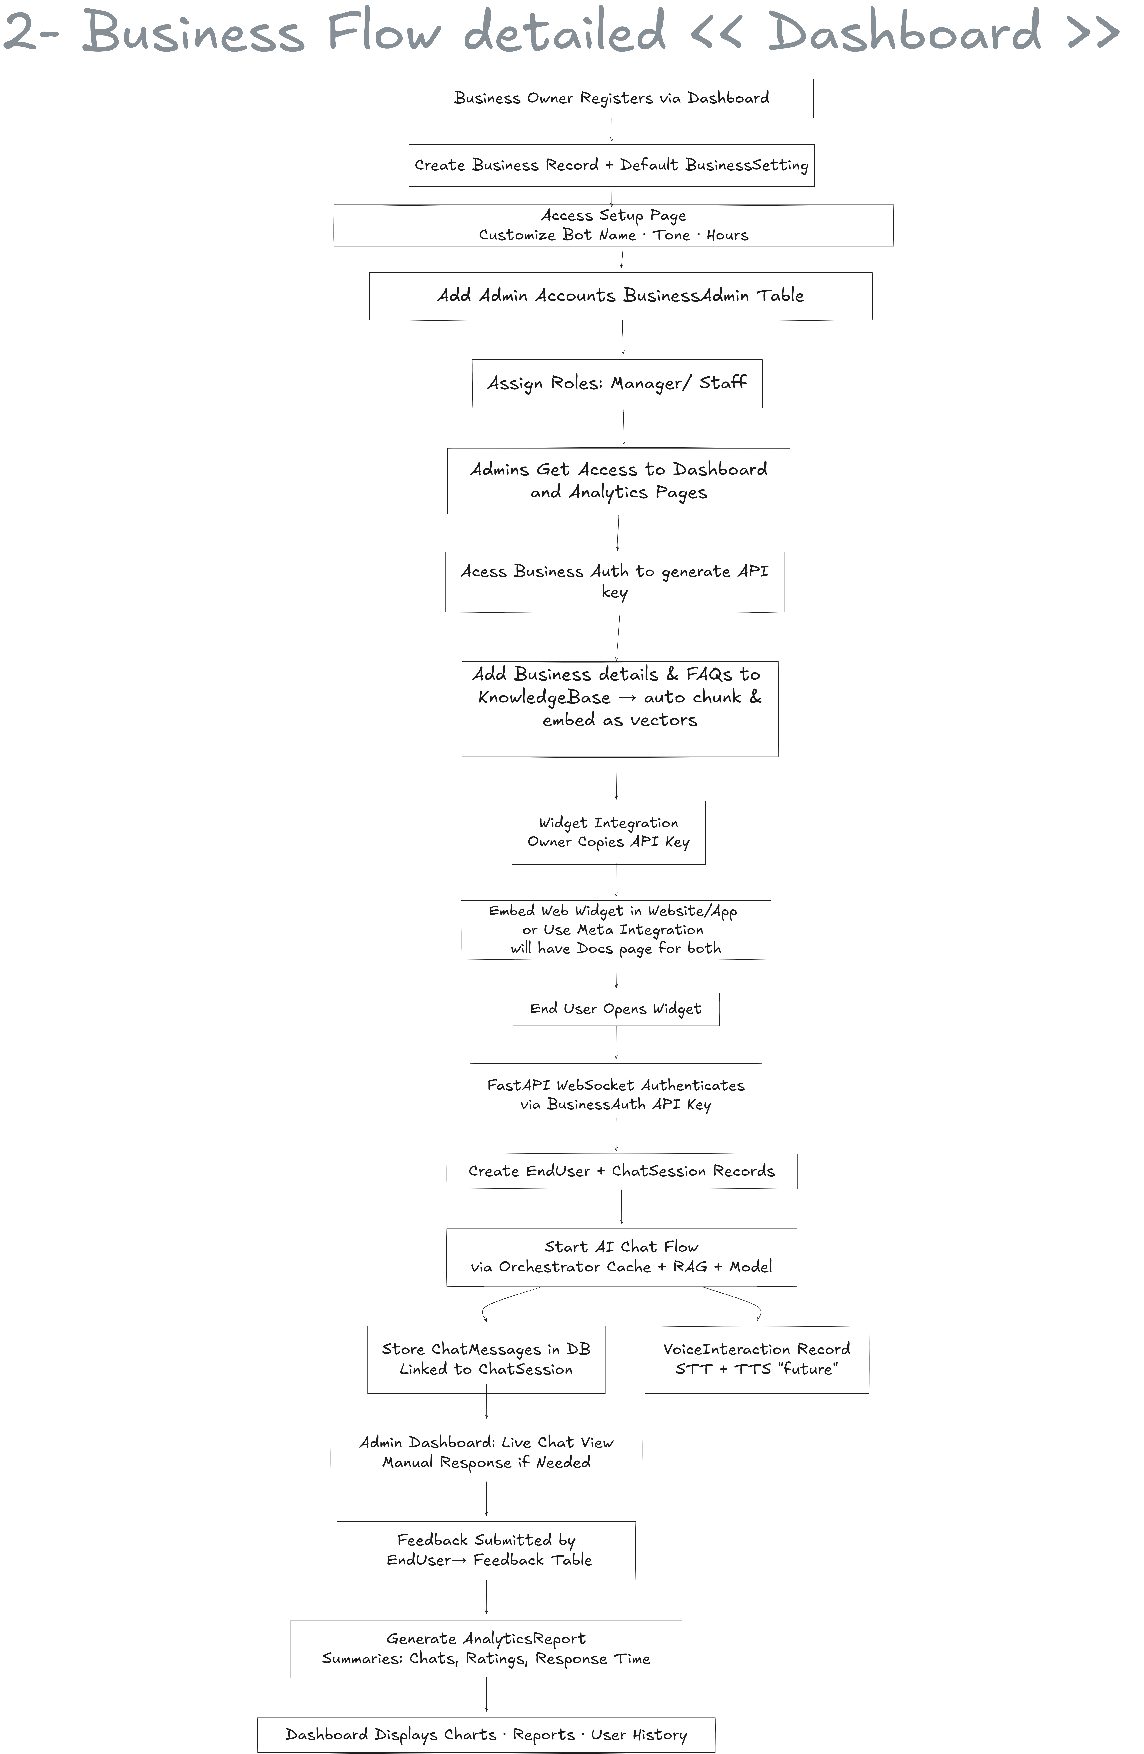
\includepdf[pages=-, fitpaper=true]{business flow.pdf}
\includepdf[pages=-, fitpaper=true]{Kalamna_ERD.pdf}
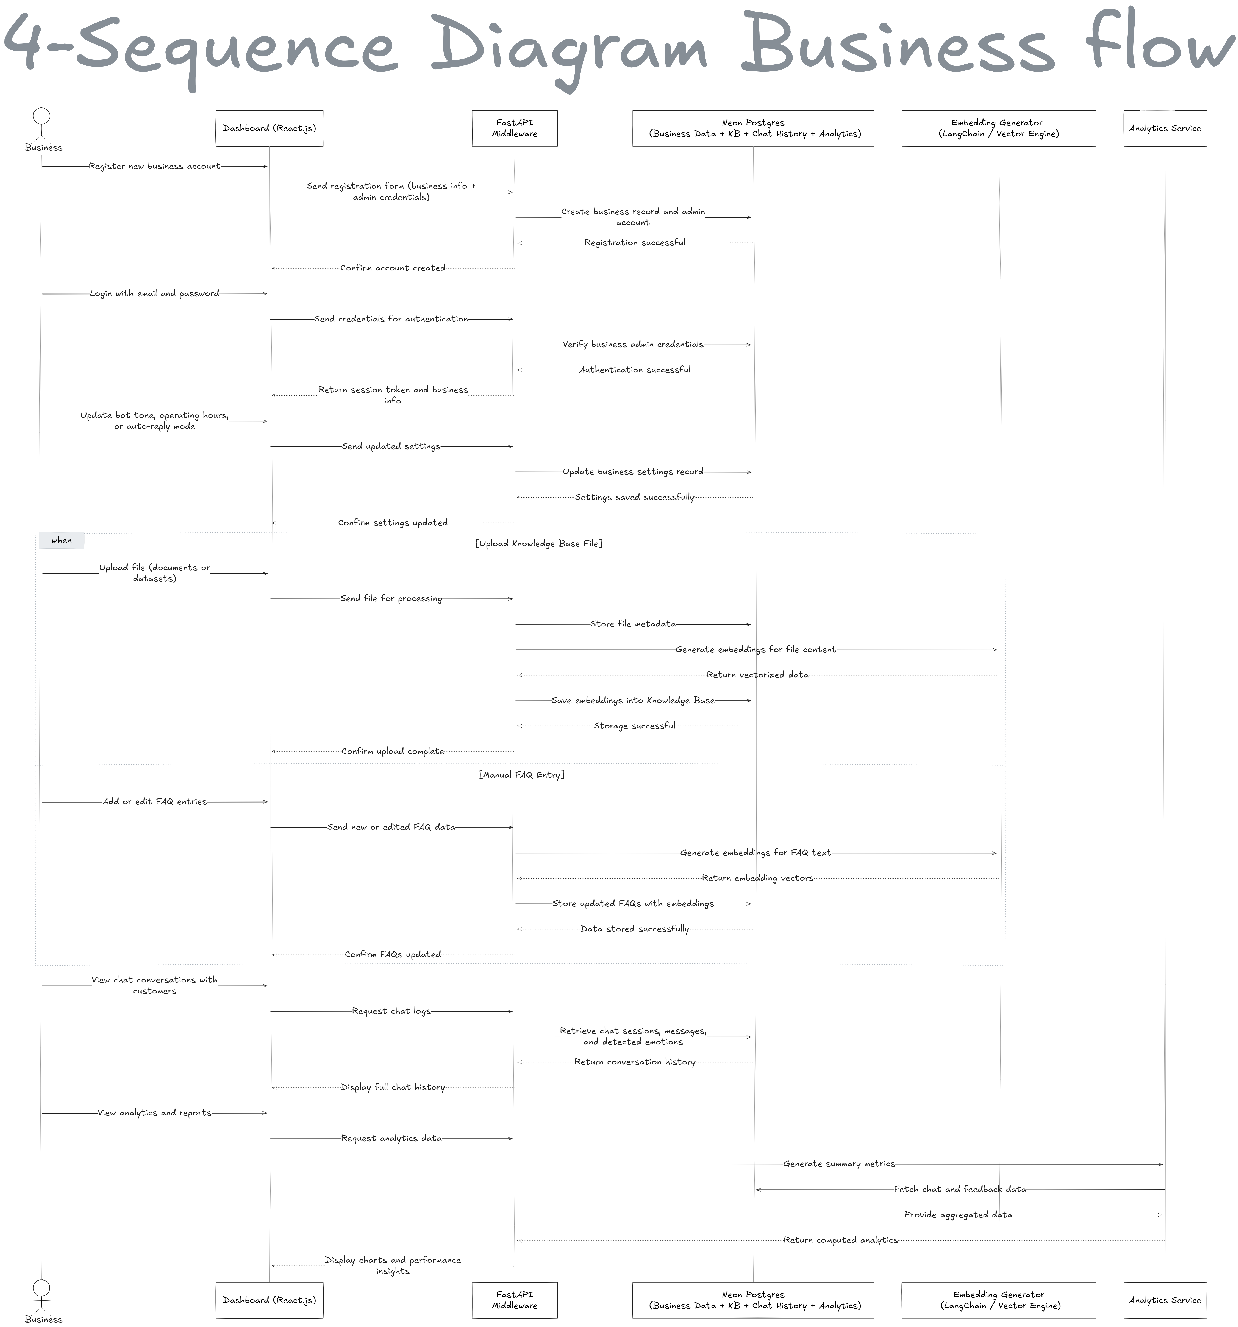
\includepdf[pages=-, fitpaper=true]{sequence diagram Business.pdf}
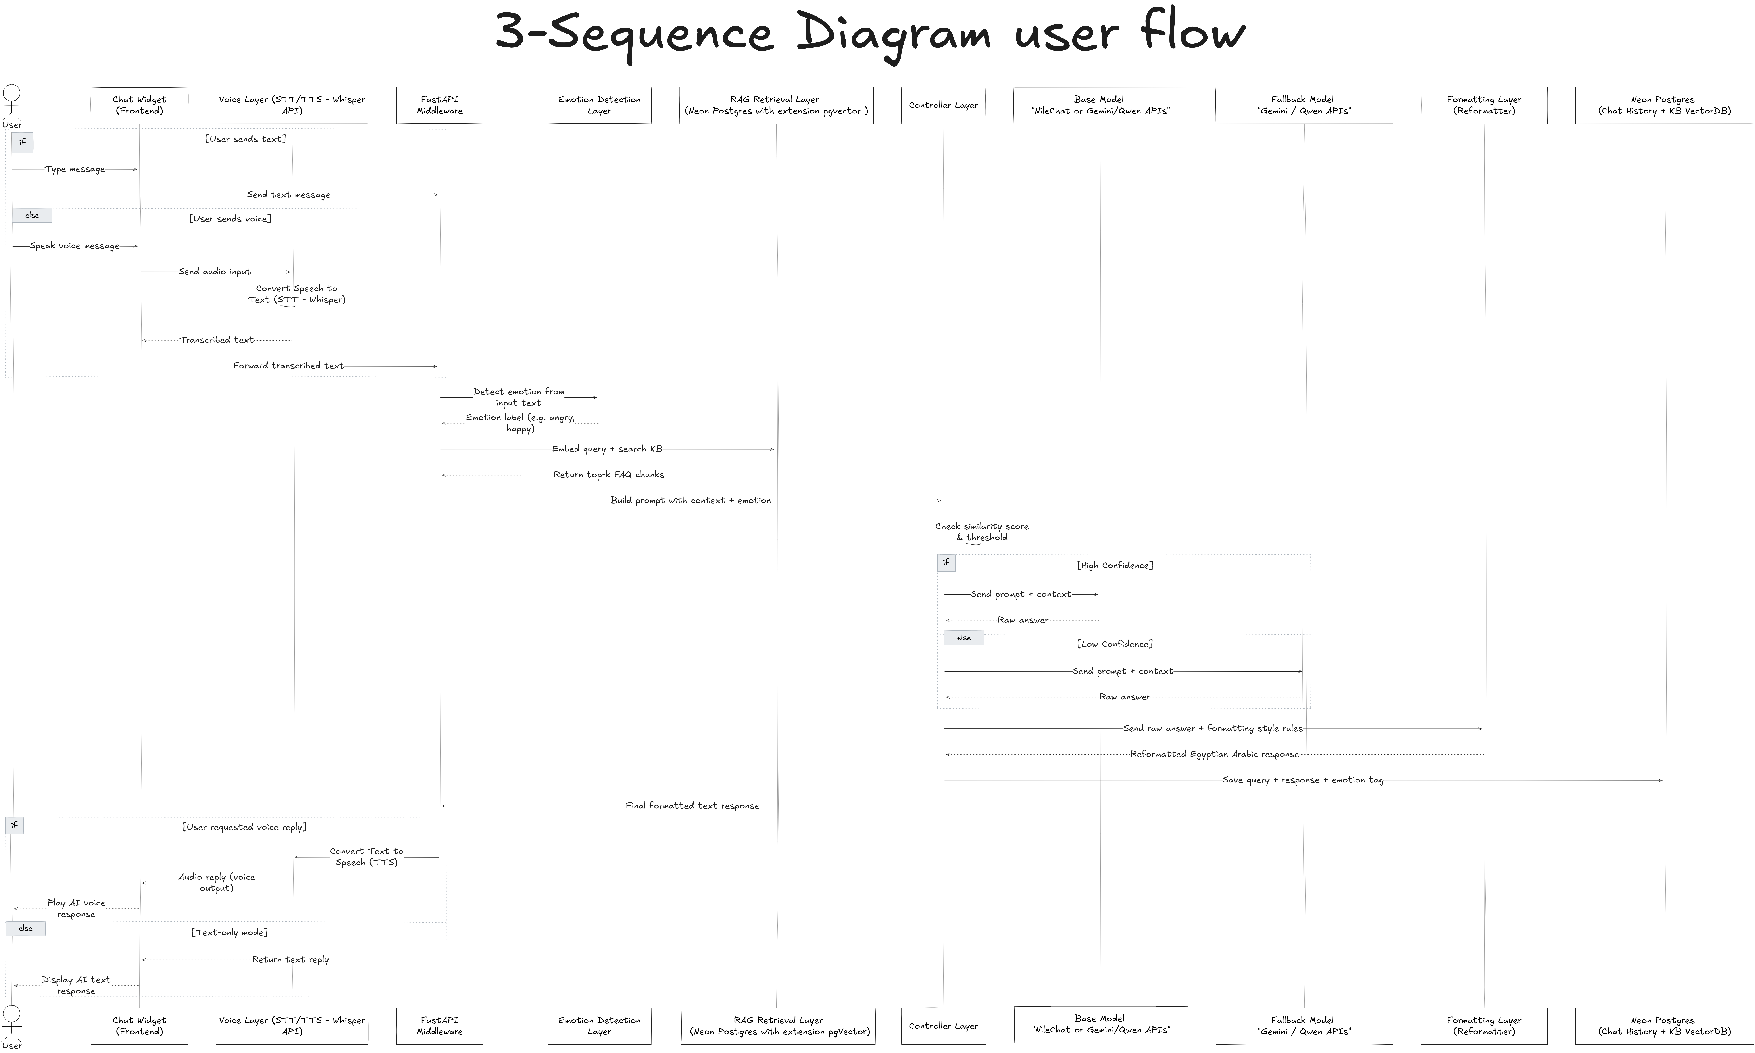
\includepdf[pages=-, fitpaper=true]{Sequence diagram user.pdf}
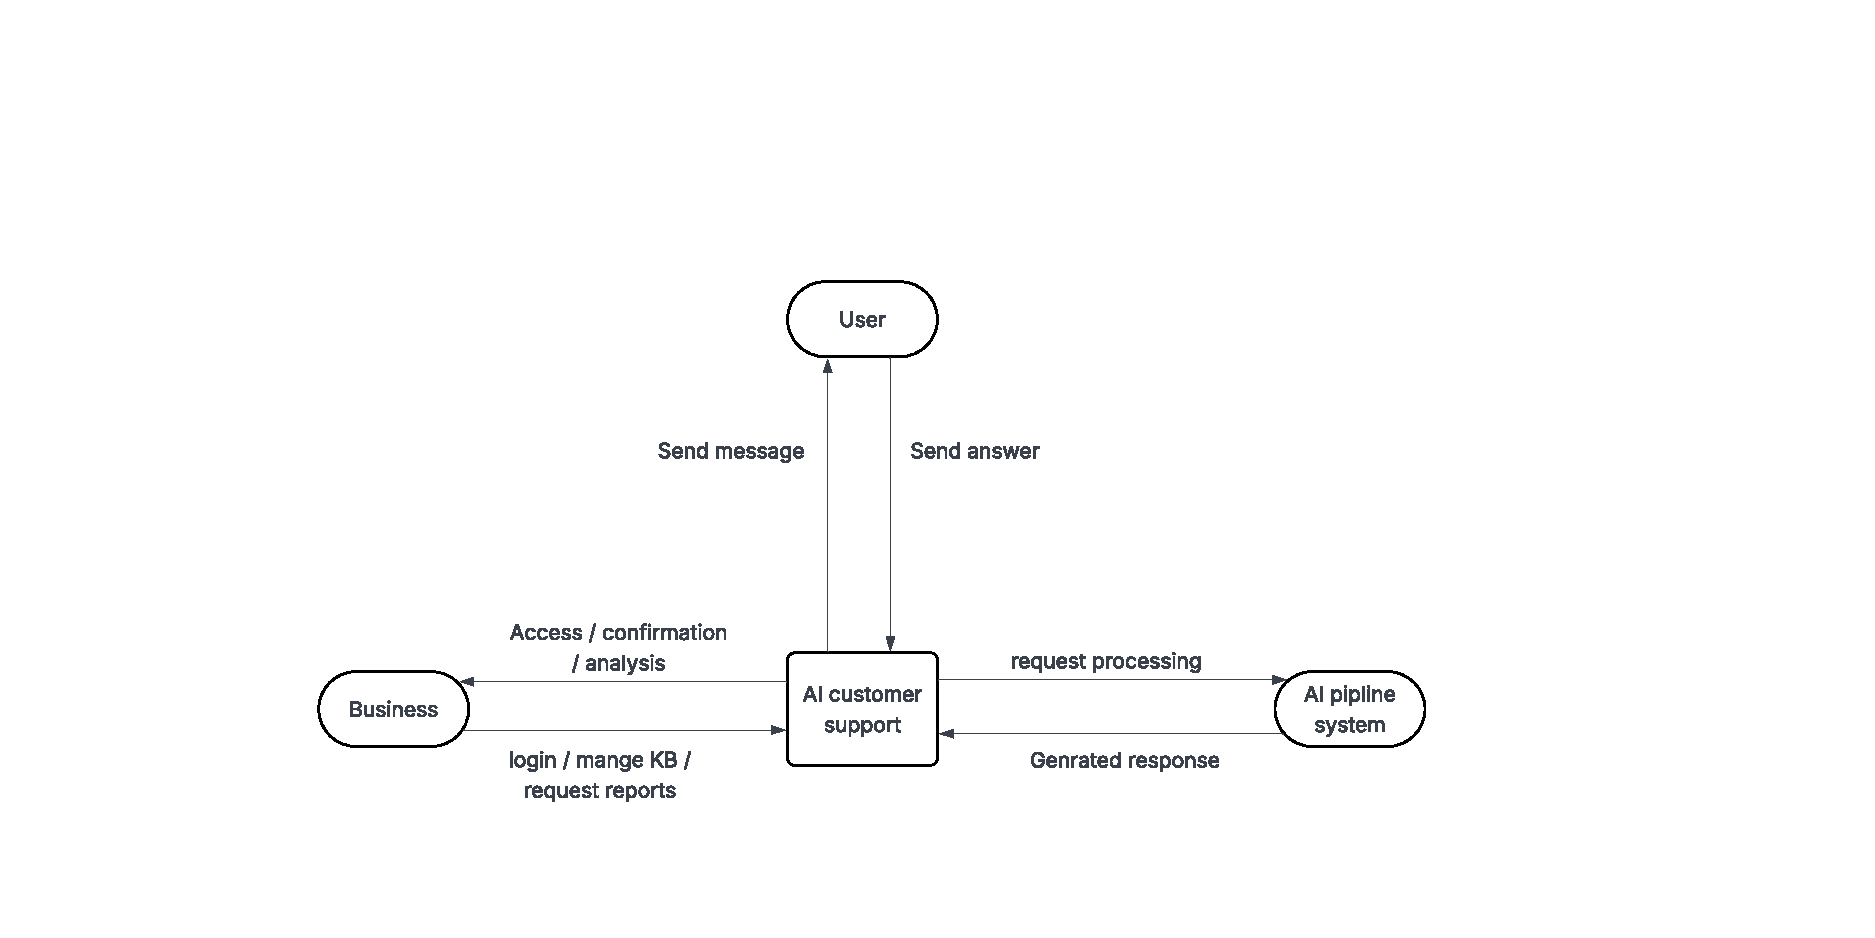
\includepdf[pages=-, fitpaper=true]{DFD level 0.pdf}
\includepdf[pages=-, fitpaper=true]{DFD level 1 user flow.pdf}
\includepdf[pages=-, fitpaper=true]{DFD level 2 user flow.pdf}
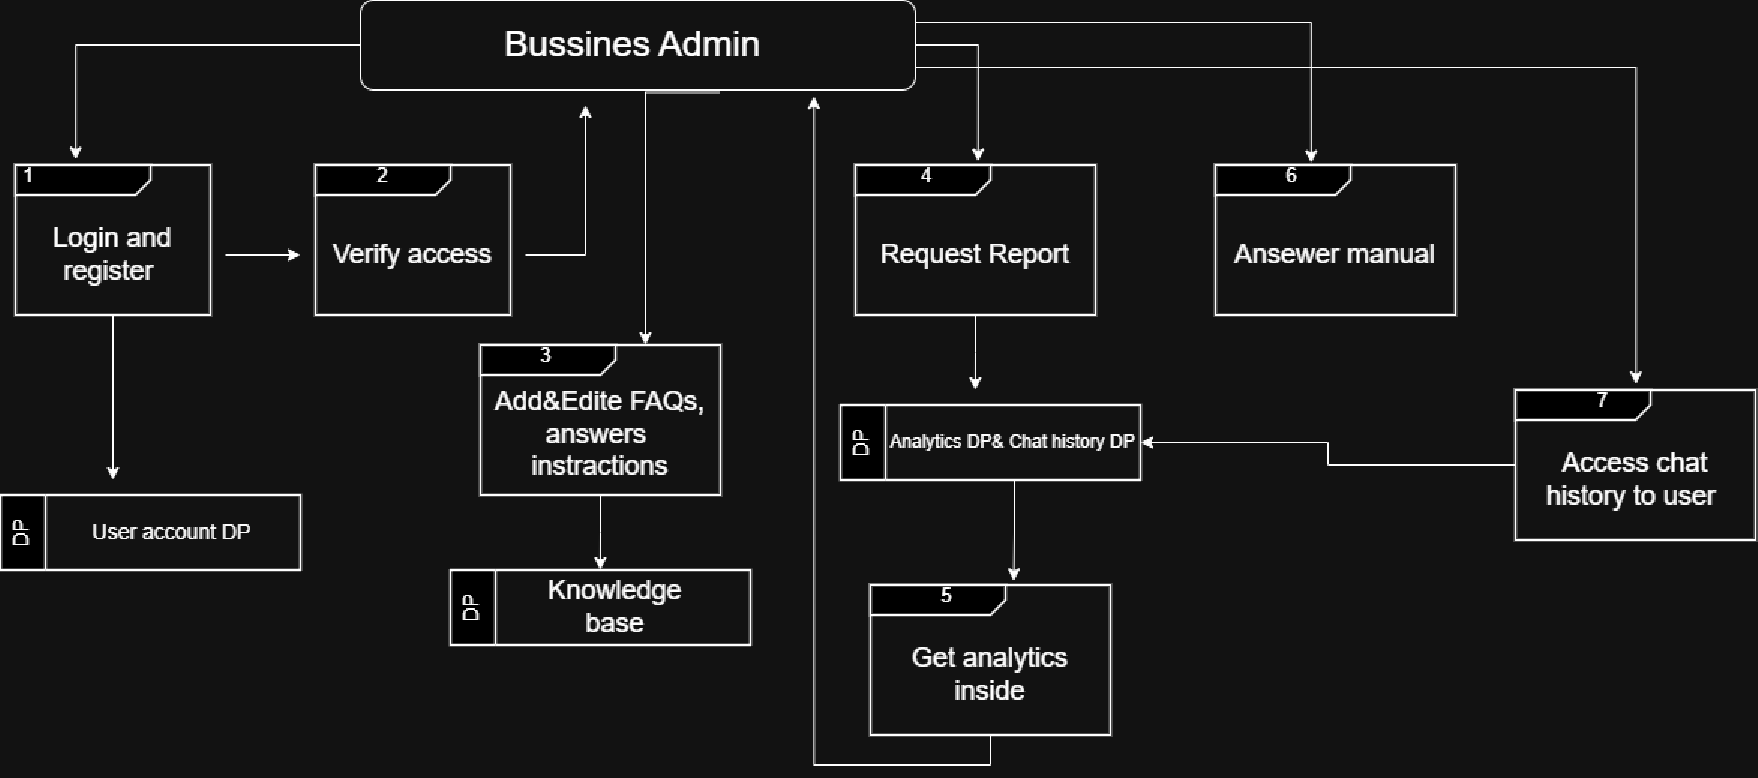
\includepdf[pages=-, fitpaper=true]{DFD Level 1 Business.pdf}
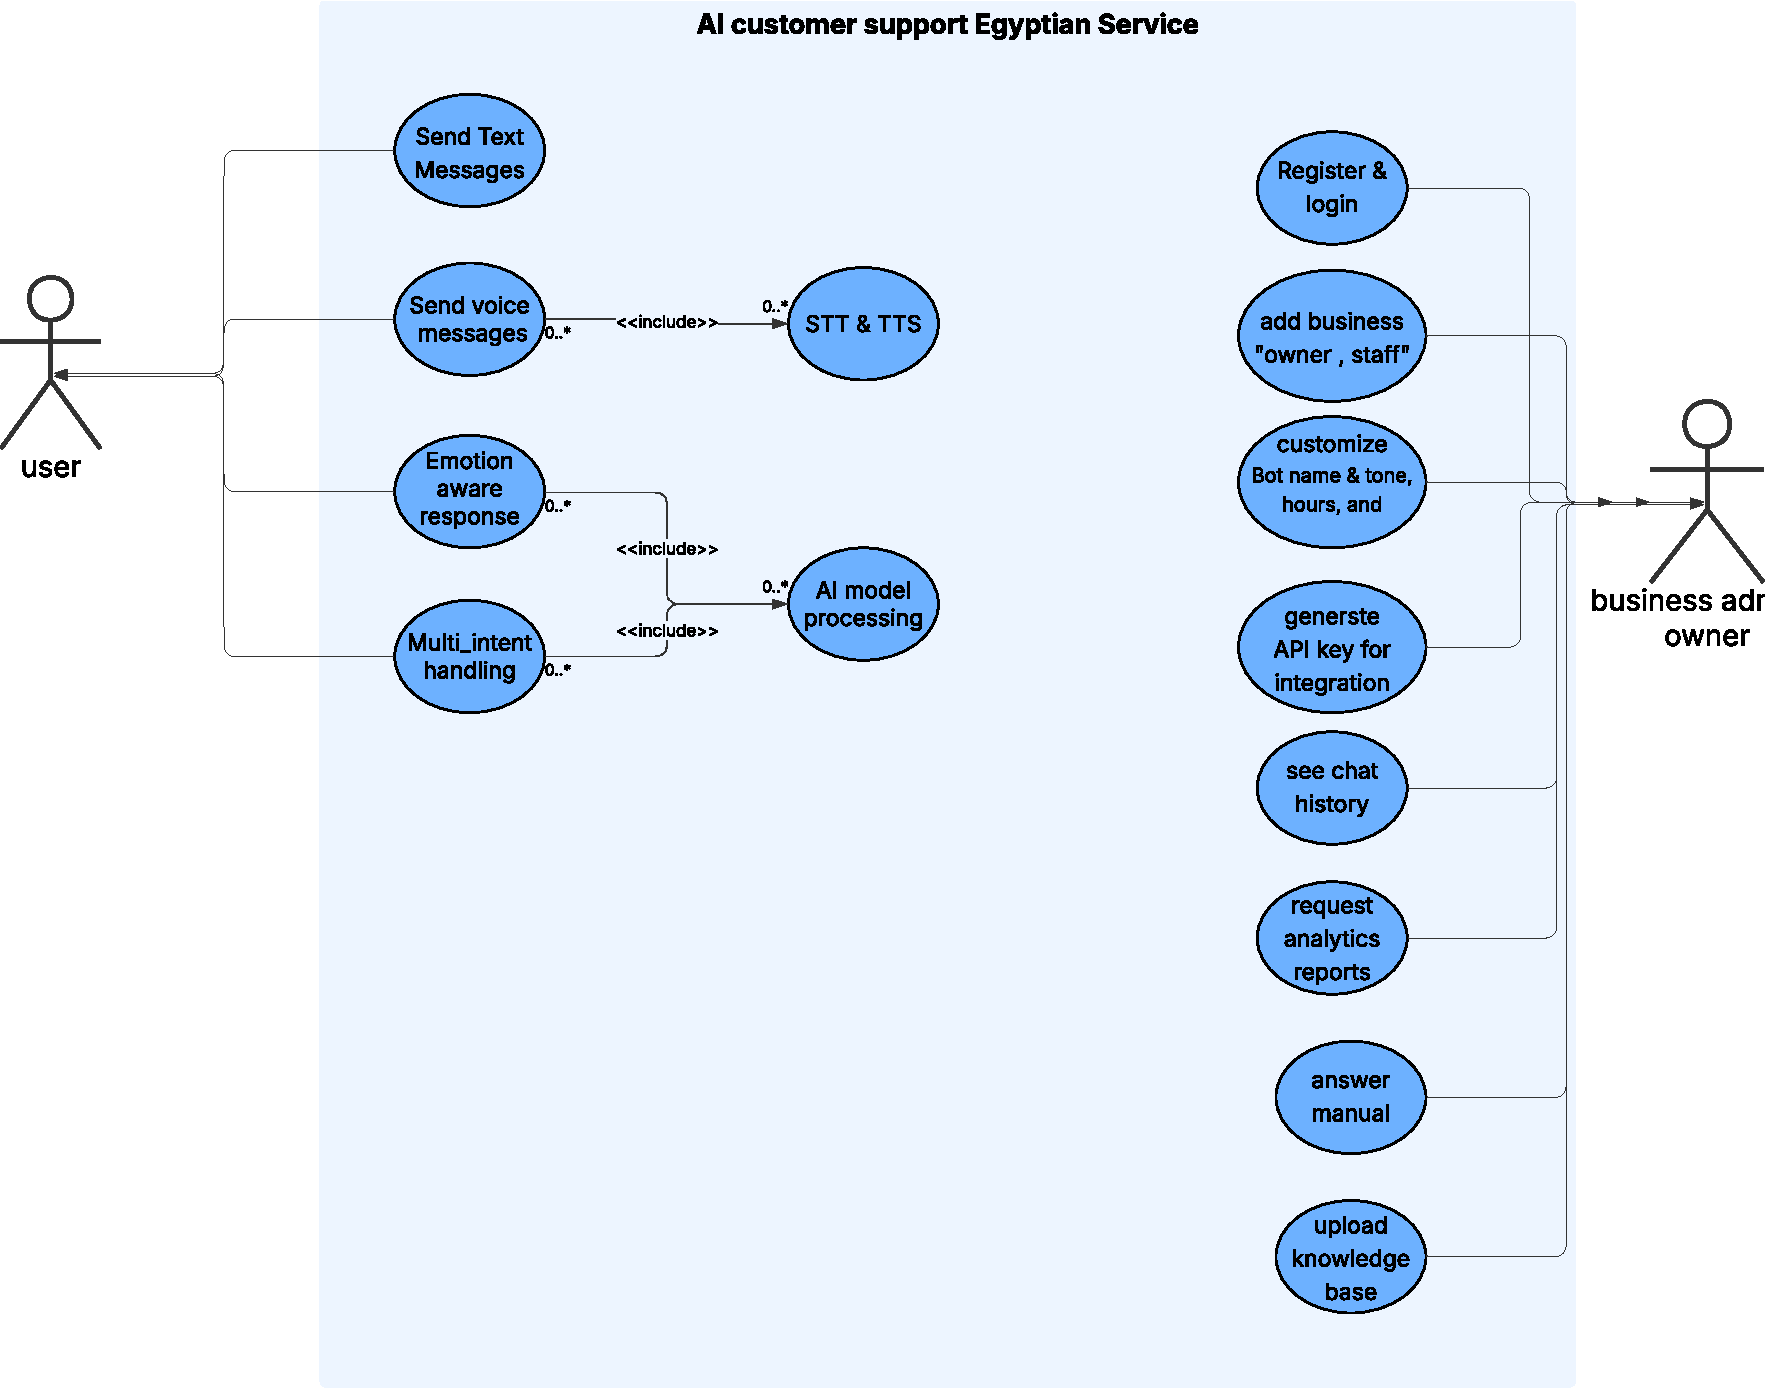
\includepdf[pages=-, fitpaper=true]{use case business and user diagram.pdf}


% ============================================================
% 5. FUNCTIONAL REQUIREMENTS SPECIFICATION (FRS)
% ============================================================
\section{Functional Requirements Specification (FRS)}
\subsection{Core Actors}

\begin{table}[H]
\centering
\renewcommand{\arraystretch}{1.3}
\begin{tabular}{|p{0.3\linewidth}|p{0.6\linewidth}|}
\hline
\textbf{Actor} & \textbf{Description} \\
\hline
End User (Customer) & A visitor or client interacting with the business chatbot via widget or Meta integration. \\
\hline
Business Admin & Registered business staff managing chatbot configurations, viewing analytics, and editing the knowledge base. \\
\hline
AI System & Orchestrator responsible for intent detection, emotion analysis, RAG retrieval, and response generation. \\
\hline
Backend API (FastAPI) & Middleware managing requests between user, AI models, and the database (PostgreSQL). \\
\hline
Database (Neon PostgreSQL + pgvector) & Stores all persistent entities: users, sessions, messages, knowledge base, and analytics reports. \\
\hline
\end{tabular}
\end{table}

\vspace{1em}
\noindent\hrulefill
\vspace{1em}

\subsection{Functional Requirements}

\subsubsection{User Interaction (Text and Voice)}
\begin{itemize}
    \item \textbf{FR1:} The system shall allow users to send \textbf{text messages} through the chat widget or Meta channels.
    \item \textbf{FR2:} The system shall support \textbf{voice input} (speech-to-text) and \textbf{voice output} (text-to-speech) via Whisper and TTS APIs (future).
    \item \textbf{FR3:} The system shall store each message or voice record in \texttt{ChatMessage} or \texttt{VoiceInteraction} with metadata such as AI model used, detected emotion, timestamp, content or transcription text, voice URL, and sender type.
    \item \textbf{FR4:} The system shall detect user \textbf{emotion} from the text or voice tone using an emotion detection layer.
    \item \textbf{FR5:} The chatbot shall \textbf{adapt its tone or response style} based on the detected emotion and business tone configuration.
\end{itemize}

\vspace{1em}
\noindent\hrulefill
\vspace{1em}

\subsubsection{Widget \& Meta Integration}
\begin{itemize}
    \item \textbf{FR6:} The system shall provide an \textbf{embeddable chat widget} using a unique \texttt{api\_key} from \texttt{BusinessAuth}.
    \item \textbf{FR7:} The widget shall support \textbf{real-time messaging}, \textbf{typing indicators}, and \textbf{session persistence}.
    \item \textbf{FR8:} The system shall verify the \texttt{api\_key} before initializing any chat session.
    \item \textbf{FR9:} The system shall integrate with \textbf{WhatsApp}, \textbf{Messenger}, and \textbf{Instagram APIs} (planned feature) for businesses to connect their customer channels.
    \item \textbf{FR10:} The widget and integrations shall automatically switch to \textbf{offline mode} outside business hours (\texttt{operating\_hour\_start} / \texttt{operating\_hour\_end}).
\end{itemize}

\vspace{1em}
\noindent\hrulefill
\vspace{1em}

\subsubsection{Knowledge Base and AI Response}
\begin{itemize}
    \item \textbf{FR11:} The business admin shall be able to upload or input \textbf{FAQs, text, or files} into the \texttt{KnowledgeBase} (text or file-based).
    \item \textbf{FR12:} The AI pipeline shall generate \textbf{embedding vectors} for each entry using AI frameworks (e.g., LangChain) and store them in the \texttt{embedding\_vector} field.
    \item \textbf{FR13:} When a user message is received, the system shall perform \textbf{contextual retrieval (RAG)} to fetch top-matching knowledge chunks.
    \item \textbf{FR14:} The AI controller layer shall choose the most confident model output between \textbf{NileChat}, \textbf{Gemini}, or \textbf{Qwen} based on similarity threshold.
    \item \textbf{FR15:} The system shall format AI responses based on business rules from \texttt{BusinessSetting}, consistently using a \textbf{response formatting layer}.
\end{itemize}

\vspace{1em}
\noindent\hrulefill
\vspace{1em}

\subsubsection{Business Registration and Authentication}
\begin{itemize}
    \item \textbf{FR16:} Businesses can register an account providing \texttt{name}, \texttt{email}, and \texttt{domain\_url}.
    \item \textbf{FR17:} A default \texttt{BusinessSetting} and active \texttt{BusinessAuth} record shall be automatically generated upon registration.
    \item \textbf{FR18:} Each business can manage multiple \texttt{BusinessAdmin} accounts with roles (\texttt{owner}, \texttt{staff}).
    \item \textbf{FR19:} Authentication shall be done through secure login using email and password.
    \item \textbf{FR20:} The system shall allow owners to \textbf{generate, rotate, or deactivate API keys} without deleting the business record.
\end{itemize}

\vspace{1em}
\noindent\hrulefill
\vspace{1em}

\subsubsection{Dashboard Management}
\begin{itemize}
    \item \textbf{FR21:} The business admin shall access an \textbf{admin dashboard} via web (React.js).
    \item \textbf{FR22:} The dashboard shall allow management of:
    \begin{itemize}
        \item Knowledge Base entries (CRUD)
        \item Bot tone style and response mode (auto/manual)
        \item Operating hours
        \item Viewing chat history and feedback
    \end{itemize}
    \item \textbf{FR23:} The dashboard shall show analytics reports such as total chats, average response time, and user satisfaction (from \texttt{AnalyticsReport}).
    \item \textbf{FR24:} The dashboard shall include a \textbf{manual reply mode}, allowing admins to respond directly to ongoing chats if AI auto-reply is disabled.
\end{itemize}

\vspace{1em}
\noindent\hrulefill
\vspace{1em}

\subsubsection{Chat Session Management}
\begin{itemize}
    \item \textbf{FR25:} When a user starts chatting, the system shall create a new \texttt{ChatSession} linked to the \texttt{EndUser} and \texttt{Business}.
    \item \textbf{FR26:} All messages within the same chat shall link to that session ID for history tracking.
    \item \textbf{FR27:} When a chat ends, the system shall mark the session as \texttt{closed} or \texttt{expired}.
    \item \textbf{FR28:} The user shall be prompted to submit \textbf{feedback} (rating and comment), stored in the \texttt{Feedback} table.
\end{itemize}

\vspace{1em}
\noindent\hrulefill
\vspace{1em}

\subsubsection{Analytics and Reporting}
\begin{itemize}
    \item \textbf{FR29:} The system shall automatically aggregate chat statistics and feedback to generate \texttt{AnalyticsReport} entries.
    \item \textbf{FR30:} Reports shall include total chats, average response time, and average user satisfaction.
    \item \textbf{FR31:} Reports shall be available for download or viewing in the dashboard.
    \item \textbf{FR32:} Analytics shall update periodically (e.g., daily or weekly background job).
\end{itemize}

\vspace{1em}
\noindent\hrulefill
\vspace{1em}

\subsubsection{Voice Interaction (Future Expansion)}
\begin{itemize}
    \item \textbf{FR33:} The system shall store voice recordings and transcription text in the \texttt{VoiceInteraction} table.
    \item \textbf{FR34:} The system shall detect emotion from voice tone and integrate results with AI response generation.
    \item \textbf{FR35:} The chatbot shall be able to \textbf{reply with customized voice} based on user preference or platform type (e.g., WhatsApp voice message).
\end{itemize}

\vspace{1em}
\noindent\hrulefill
\vspace{1em}

\subsubsection{AI Pipeline Orchestration}
\begin{itemize}
    \item \textbf{FR36:} The AI Orchestrator shall manage the workflow between input message $\rightarrow$ emotion detection $\rightarrow$ RAG $\rightarrow$ model selection $\rightarrow$ formatting $\rightarrow$ output.
    \item \textbf{FR37:} The orchestrator shall fallback between models if the primary fails.
    \item \textbf{FR38:} Each step of the pipeline shall log its operation (model used, latency, confidence score).
\end{itemize}

\vspace{1em}
\noindent\hrulefill
\vspace{1em}

\subsubsection{System Administration}
\begin{itemize}
    \item \textbf{FR39:} The system shall maintain logs of authentication attempts, API usage, and integration events.
    \item \textbf{FR40:} The system shall support environment-based configurations for development, staging, and production.
    \item \textbf{FR41:} The system shall notify admins of integration errors (e.g., API key invalid, channel disconnected).
\end{itemize}

\section{Non-Functional Requirements}

\subsection{Performance}

\begin{itemize}[leftmargin=2cm]
    \item \textbf{NFR-1:} Average chatbot response (text) shall be less than or equal to \textbf{5 seconds} for 90\% of requests.
    \item \textbf{NFR-2:} Emotion detection latency shall not exceed \textbf{600 ms for text , 1000ms for voice}, and RAG retrieval shall not exceed \textbf{1.5 s for text , 3 s for voice}.
    \item \textbf{NFR-3:} Voice query processing (audio → text → reply) shall take less than 1 min
    \item \textbf{NFR-4:} Average database query latency shall not exceed \textbf{200 ms} under normal load.
\end{itemize}

\subsection{Scalability}

\begin{itemize}[leftmargin=2cm]
    \item \textbf{NFR-5:} The architecture shall support \textbf{horizontal scaling} using Docker and (Railway or Coolify) .
    \item \textbf{NFR-6:} The queue system (Redis "caching") shall buffer up to \textbf{2k concurrent jobs} without failure.
\end{itemize}

\subsection{ Reliability \& Availability}

\begin{itemize}[leftmargin=2cm]
    \item \textbf{NFR-7:} The system shall maintain an uptime of at least \textbf{95\% per month}.
    \item \textbf{NFR-8:} Critical services shall automatically restart within \textbf{30 seconds} after failure.
    \item \textbf{NFR-9:} Database backups shall be taken \textbf{daily} and retained for \textbf{14 days}.
    \item \textbf{NFR-10:} Model fallback (NileChat → Gemini → Qwen) success rate shall be at least \textbf{95\%}.
\end{itemize}

\subsection{ Security}

\begin{itemize}[leftmargin=2cm]
    \item \textbf{NFR-11:} All traffic shall use \textbf{HTTPS/TLS 1.3}.
\item \textbf{NFR-12:} Passwords shall be hashed using \textbf{bcrypt (cost $\geq$ 12)}, and API keys hashed using \textbf{SHA-256}.

    \item \textbf{NFR-13:} JWT access tokens shall expire in \textbf{24 hours}, and refresh tokens shall be valid for \textbf{7 days}.
    \item \textbf{NFR-14:} Accounts shall be locked after \textbf{5 failed login attempts within 30 minutes}.
    \item \textbf{NFR-15:} Sensitive data shall be encrypted at rest using \textbf{AES-256}.
\end{itemize}

\subsection{ Usability}

\begin{itemize}[leftmargin=2cm]
    \item \textbf{NFR-16:} Chat widget shall load in less than or equal to \textbf{30 seconds}
    \item \textbf{NFR-17:} Dashboard shall be responsive for screens wider than \textbf{768 px}.
    \item \textbf{NFR-18:} System shall support both \textbf{Arabic (Egyptian dialect)} and \textbf{English}, with automatic RTL layout.
    \item \textbf{NFR-19:} At least \textbf{80\% of users} shall be able to complete a chat without assistance
\end{itemize}

\subsection{Maintainability \& Testability}

\begin{itemize}[leftmargin=2cm]
    \item \textbf{NFR-20:} Codebase shall be organized into modular components: \texttt{api}, \texttt{ai\_pipeline}, \texttt{db}, \texttt{dashboard}, and \texttt{integrations}.
    \item \textbf{NFR-21:} Unit-test coverage shall be at least \textbf{70\%} for backend components.
    \item \textbf{NFR-22:} The CI/CD pipeline (GitHub Actions) shall complete build and deployment in less than \textbf{8 minutes}.
    \item \textbf{NFR-23:} All APIs shall include auto-generated documentation using \textbf{Swagger} or \textbf{ReDoc} and manual postman doc for testing.
\end{itemize}

\subsection{Observability}

\begin{itemize}[leftmargin=2cm]
    \item \textbf{NFR-24:} JSON logs shall be generated for every API call and AI model latency.
    \item \textbf{NFR-25:} Critical system errors shall trigger alerts (via slack or email ) within \textbf{5 minutes} of detection.
\end{itemize}

\subsection{Privacy}

\begin{itemize}[leftmargin=2cm]
    \item \textbf{NFR-26:} The system shall comply with \textbf{Egyptian Data Protection Law}.
    \item \textbf{NFR-27:} Minimal personal data shall be stored, and identifiers shall be hashed or pseudonymized.
    \item \textbf{NFR-28:} Businesses shall be able to export or delete their stored data.
\end{itemize}


% ============================================================
% RISK ANALYSIS
% ============================================================
\section{Risk Analysis Plan}

\renewcommand{\arraystretch}{1.3}

\begin{table}[H]
\centering
\begin{tabularx}{\textwidth}{
    >{\bfseries}l  % Bold category
    X               % Description (stretch)
    c               % Probability
    c               % Impact
    X               % Mitigation
}
\toprule
Category & Risk Description & Probability & Impact & Mitigation / Prevention \\
\midrule

Technical & AI model integration (Gemini / GPT / NileChat) may fail or produce inconsistent outputs. & Medium & High & Create a fallback layer with multiple models and strong prompt formatting. \\

\addlinespace
Data Quality & Poor or insufficient Egyptian Arabic datasets for training emotion detection or intent models. & High & High & Use open datasets, fine-tuning, and real testing with SMEs. \\

\addlinespace
Performance & Chatbot may experience slow response time or overload under concurrent users. & Medium & Medium & Optimize backend performance using async, caching, and monitoring tools. \\

\addlinespace
Security & Unauthorized access to business data or chat logs. & Medium & High & Implement JWT, encryption, and role-based access controls. \\

\addlinespace
User Acceptance & Businesses may find customization complex or prefer competitors. & Medium & High & Simplify dashboard UI and emphasize SME-friendly pricing. \\

\addlinespace
Financial & Budget or sponsorship delays. & Low & Medium & Use minimal-cost deployment options and open-source resources. \\

\addlinespace
Ethical / Legal & Issues with data privacy and user consent. & Low & High & Ensure consent-based data usage and anonymize logs. \\

\bottomrule
\end{tabularx}
\caption{Risk Analysis Plan for the AI Customer Support Platform}
\label{tab:risk_analysis}
\end{table}
\section{Security Implementation Plan}
Security is integrated across all project phases and layers to ensure the chatbot platform remains safe, compliant, and resilient against real-world threats. The security design aligns with OWASP Top 10 and modern AI system protection standards.

\subsection{Security Objectives}
\begin{itemize}
    \item Protect user and business data during storage, processing, and communication.
    \item Prevent unauthorized access or abuse through robust authentication and rate limiting.
    \item Ensure AI and API components cannot be exploited or injected with malicious inputs.
    \item Maintain system visibility and control through secure logging and monitoring.
\end{itemize}

\subsection{Implementation Details}
\subsubsection{1. Authentication \& Authorization}
\begin{itemize}
    \item Implement OAuth2 and JWT-based authentication for all users and businesses.
    \item Use short-lived tokens and refresh mechanisms to prevent token reuse.
    \item Enforce Role-Based Access Control (RBAC) for business admins and platform users.
\end{itemize}

\subsubsection{2. Data Protection}
\begin{itemize}
    \item Enforce HTTPS/TLS for all communication (frontend, backend, APIs, integrations).
    \item Encrypt sensitive data (chat logs, credentials, business info) in PostgreSQL (pgcrypto).
    \item Use environment variables and secret management in CI/CD to protect API keys.
\end{itemize}

\subsubsection{3. Input Validation \& AI Security}
\begin{itemize}
    \item Validate and sanitize all user inputs with Pydantic schemas.
    \item Prevent prompt injection and ensure AI models only access intended data.
    \item Filter and review AI responses before displaying them to users.
\end{itemize}

\subsubsection{4. API \& Network Security}
\begin{itemize}
    \item Apply rate limiting and throttling on key endpoints to prevent abuse.
    \item Enforce CORS with domain whitelisting for integrations (WhatsApp, Facebook, Web).
    \item Use Docker container isolation and vulnerability scans (Trivy, Bandit).
\end{itemize}

\subsubsection{5. Monitoring \& Testing}
\begin{itemize}
    \item Enable structured security logging (Loguru) for authentication and API events.
    \item Mask sensitive data in logs.
    \item Automate OWASP ZAP and Bandit scans in GitHub CI/CD pipeline.
    \item Conduct periodic penetration testing and performance checks before release.
\end{itemize}

\subsection{OWASP Top 10 Security Measures}

\subsubsection{1. Authentication \& Session Security (A07: Identification \& Authentication Failures)}
Already covered: OAuth2 + JWT.

\textbf{Add:}
\begin{itemize}
    \item Token rotation \& short TTL (short-lived JWTs, refresh tokens stored securely).
    \item Device/session revocation — allow logout from all sessions.
    \item Secure password policy + account lockout on repeated failed logins.
    \item Use FastAPI’s OAuth2PasswordBearer securely (no token in URL).
\end{itemize}

\subsubsection{2. Access Control \& Authorization (A01: Broken Access Control)}
\begin{itemize}
    \item Enforce RBAC (Role-Based Access Control) between businesses, admins, and normal users.
    \item Prevent access to chat histories or admin routes unless authorized.
    \item Use path- and object-level access control (e.g., users can only view their own chat logs).
    \item Validate all incoming API requests against permissions.
\end{itemize}

\subsubsection{3. Data Protection \& Privacy (A02: Cryptographic Failures)}
\begin{itemize}
    \item Encrypt sensitive data (e.g., chat logs, business info) in PostgreSQL using pgcrypto.
    \item Never store plain tokens, passwords, or API keys.
    \item Use \texttt{.env} for credentials (never hardcode).
    \item Force HTTPS for all communications, including AI API calls.
\end{itemize}

\subsubsection{4. Injection \& Input Validation (A03: Injection, A05: Security Misconfiguration)}
\begin{itemize}
    \item Sanitize all incoming user messages before processing (no injection into AI prompts).
    \item Use parameterized queries in PostgreSQL.
    \item Add input schema validation in FastAPI with Pydantic.
    \item Escape all user-provided content on the frontend (prevent XSS).
    \item Filter file uploads (if added later) by MIME type.
\end{itemize}

\subsubsection{5. Prompt Injection \& AI Layer Security (Emerging Category, OWASP LLM Top 10)}
Since you’re using LLMs (Gemini/Qwen):
\begin{itemize}
    \item Implement input/output sanitization before passing data to AI.
    \item Restrict model access to only what’s needed (no sensitive data in prompts).
    \item Add a safety layer that checks responses before returning them to users.
    \item Limit what the AI can access through LangChain (no unrestricted file or system calls).
\end{itemize}

\subsubsection{6. API Security (A08: Software and Data Integrity Failures)}
\begin{itemize}
    \item Require API keys or OAuth2 for external integrations (WhatsApp, Facebook, etc.).
    \item Add Rate Limiting + Throttling per endpoint.
    \item Use CORS with strict domain whitelisting.
    \item Validate all payloads with schemas (avoid mass assignment vulnerabilities).
\end{itemize}

\subsubsection{7. Dependency \& Infrastructure Security (A06: Vulnerable \& Outdated Components)}
\begin{itemize}
    \item Use Dependabot or Safety CLI to scan dependencies weekly.
    \item Regularly update FastAPI, React, and Hugging Face libraries.
    \item Keep Docker images minimal and use non-root users.
    \item Scan Docker images for vulnerabilities (e.g., Trivy).
\end{itemize}

\subsubsection{8. Logging \& Monitoring (A09: Security Logging \& Monitoring Failures)}
\begin{itemize}
    \item Implement structured logging (e.g., Loguru in FastAPI).
    \item Log all login attempts, API errors, and suspicious activity.
    \item Mask sensitive data in logs (tokens, passwords).
    \item Set up alerting on failed login bursts or rate-limit triggers.
\end{itemize}

\subsubsection{9. Server \& Config Security (A05: Security Misconfiguration)}
\begin{itemize}
    \item Enforce Content Security Policy (CSP) in React.
    \item Disable directory listing and debug mode.
    \item Use secure headers (HSTS, X-Frame-Options, X-Content-Type-Options).
    \item Manage secrets securely (GitHub Actions Secrets + .env + Docker secrets).
\end{itemize}

\subsubsection{10. Business Logic \& Abuse Prevention (A10: SSRF, A04: Insecure Design)}
\begin{itemize}
    \item Validate that bots can’t be abused to spam or flood messages.
    \item Limit AI response length and frequency.
    \item Validate business IDs and message origins.
    \item Use rate limiting per user/IP to stop abuse of free tiers or spam attacks.
\end{itemize}

\end{document}
